\documentclass[twoside]{book}

% Packages required by doxygen
\usepackage{fixltx2e}
\usepackage{calc}
\usepackage{doxygen}
\usepackage[export]{adjustbox} % also loads graphicx
\usepackage{graphicx}
\usepackage[utf8]{inputenc}
\usepackage{makeidx}
\usepackage{multicol}
\usepackage{multirow}
\PassOptionsToPackage{warn}{textcomp}
\usepackage{textcomp}
\usepackage[nointegrals]{wasysym}
\usepackage[table]{xcolor}

% Font selection
\usepackage[T1]{fontenc}
\usepackage[scaled=.90]{helvet}
\usepackage{courier}
\usepackage{amssymb}
\usepackage{sectsty}
\renewcommand{\familydefault}{\sfdefault}
\allsectionsfont{%
  \fontseries{bc}\selectfont%
  \color{darkgray}%
}
\renewcommand{\DoxyLabelFont}{%
  \fontseries{bc}\selectfont%
  \color{darkgray}%
}
\newcommand{\+}{\discretionary{\mbox{\scriptsize$\hookleftarrow$}}{}{}}

% Page & text layout
\usepackage{geometry}
\geometry{%
  a4paper,%
  top=2.5cm,%
  bottom=2.5cm,%
  left=2.5cm,%
  right=2.5cm%
}
\tolerance=750
\hfuzz=15pt
\hbadness=750
\setlength{\emergencystretch}{15pt}
\setlength{\parindent}{0cm}
\setlength{\parskip}{3ex plus 2ex minus 2ex}
\makeatletter
\renewcommand{\paragraph}{%
  \@startsection{paragraph}{4}{0ex}{-1.0ex}{1.0ex}{%
    \normalfont\normalsize\bfseries\SS@parafont%
  }%
}
\renewcommand{\subparagraph}{%
  \@startsection{subparagraph}{5}{0ex}{-1.0ex}{1.0ex}{%
    \normalfont\normalsize\bfseries\SS@subparafont%
  }%
}
\makeatother

% Headers & footers
\usepackage{fancyhdr}
\pagestyle{fancyplain}
\fancyhead[LE]{\fancyplain{}{\bfseries\thepage}}
\fancyhead[CE]{\fancyplain{}{}}
\fancyhead[RE]{\fancyplain{}{\bfseries\leftmark}}
\fancyhead[LO]{\fancyplain{}{\bfseries\rightmark}}
\fancyhead[CO]{\fancyplain{}{}}
\fancyhead[RO]{\fancyplain{}{\bfseries\thepage}}
\fancyfoot[LE]{\fancyplain{}{}}
\fancyfoot[CE]{\fancyplain{}{}}
\fancyfoot[RE]{\fancyplain{}{\bfseries\scriptsize Generated by Doxygen }}
\fancyfoot[LO]{\fancyplain{}{\bfseries\scriptsize Generated by Doxygen }}
\fancyfoot[CO]{\fancyplain{}{}}
\fancyfoot[RO]{\fancyplain{}{}}
\renewcommand{\footrulewidth}{0.4pt}
\renewcommand{\chaptermark}[1]{%
  \markboth{#1}{}%
}
\renewcommand{\sectionmark}[1]{%
  \markright{\thesection\ #1}%
}

% Indices & bibliography
\usepackage{natbib}
\usepackage[titles]{tocloft}
\setcounter{tocdepth}{3}
\setcounter{secnumdepth}{5}
\makeindex

% Hyperlinks (required, but should be loaded last)
\usepackage{ifpdf}
\ifpdf
  \usepackage[pdftex,pagebackref=true]{hyperref}
\else
  \usepackage[ps2pdf,pagebackref=true]{hyperref}
\fi
\hypersetup{%
  colorlinks=true,%
  linkcolor=blue,%
  citecolor=blue,%
  unicode%
}

% Custom commands
\newcommand{\clearemptydoublepage}{%
  \newpage{\pagestyle{empty}\cleardoublepage}%
}

\usepackage{caption}
\captionsetup{labelsep=space,justification=centering,font={bf},singlelinecheck=off,skip=4pt,position=top}

%===== C O N T E N T S =====

\begin{document}

% Titlepage & ToC
\hypersetup{pageanchor=false,
             bookmarksnumbered=true,
             pdfencoding=unicode
            }
\pagenumbering{alph}
\begin{titlepage}
\vspace*{7cm}
\begin{center}%
{\Large vincent }\\
\vspace*{1cm}
{\large Generated by Doxygen 1.8.13}\\
\end{center}
\end{titlepage}
\clearemptydoublepage
\pagenumbering{roman}
\tableofcontents
\clearemptydoublepage
\pagenumbering{arabic}
\hypersetup{pageanchor=true}

%--- Begin generated contents ---
\chapter{Meeting}
\label{md_metting}
\Hypertarget{md_metting}
\subsection*{18\+:00\+:00 01.\+05.\+2019}

\subsubsection*{Keyword}


\begin{DoxyItemize}
\item \mbox{[}x\mbox{]} C\+Make
\item \mbox{[}x\mbox{]} clang-\/format
\item \mbox{[}x\mbox{]} app source files
\item \mbox{[}x\mbox{]} protobuf
\item \mbox{[}x\mbox{]} libhttp -\/$>$ libcurl
\item \mbox{[}x\mbox{]} log spdlog -\/$>$ spdlog \subsection*{18\+:\+:00\+:00 18.\+05.\+2019}
\end{DoxyItemize}

\subsubsection*{last metting}


\begin{DoxyItemize}
\item libhttp

add a sub-\/directory {\ttfamily http} in {\ttfamily src} directory, wrapp {\ttfamily libcurl}
\item log

add subdirectoy \textquotesingle{}log\textquotesingle{} in {\ttfamily src} directory, warapp {\ttfamily spdlog}
\end{DoxyItemize}

\subsubsection*{Keyword}


\begin{DoxyItemize}
\item \mbox{[} \mbox{]} libhttp
\item \mbox{[} \mbox{]} liblog 
\end{DoxyItemize}
\chapter{Project overview}
\label{md_overview}
\Hypertarget{md_overview}
\subsection*{Managerment}

C\+Make
\begin{DoxyItemize}
\item app
\item lib1
\item lib2
\item ...
\end{DoxyItemize}

\subsection*{Code style}

google style, cppcheck, clang-\/formt

.clang format copy from\href{https://github.com/google/jsonnet/blob/master/.clang-format}{\tt .clang-\/format} \subsection*{Comment}

doxygen \subsection*{Languange}

Cpp

\subsection*{Protocol}

Protobuf will be used for internal usage

\subsection*{Data flow}

\href{https://docs.google.com/document/d/1v2jsXLpF7iKs91sIN9Z-M3vjNxYJjjfaGAXDTr3JBIs/edit?usp=sharing}{\tt online discuss}

\subsection*{Function distribute}


\begin{DoxyItemize}
\item app

main function, service entry
\item liblog

log library spdlog, glog...
\item parse

parse input data from user input through input
\item analysis

analysis user input
\item database access
\begin{DoxyItemize}
\item abstract interface
\item each kind of datanae impletemnt the interface
\item libdba, Data\+Base\+Acces
\end{DoxyItemize}
\item libquery

convert user query to sql query command
\item libdatagenerator

construct data for client\textquotesingle{}s query
\item libhttp

find a open-\/source http lib
\item libimport$\ast$

import data from database
\item libclean$\ast$

clean data imported from database
\item libexplore$\ast$

explore analysis data from data base
\item libanalysis$\ast$

in-\/depth analysis of data from database
\item libmodel$\ast$

create model from database
\item librepresent$\ast$

create representation for data.
\end{DoxyItemize}

library name with $\ast$ is tempory, may delete in later versions, don\textquotesingle{}t rely on this. 
\chapter{Vincent}
\label{md_README}
\Hypertarget{md_README}
\href{https://app.codacy.com/app/maidamai0/vincent?utm_source=github.com&utm_medium=referral&utm_content=advanced-data-processing-company/vincent&utm_campaign=Badge_Grade_Settings}{\tt } \href{https://travis-ci.org/advanced-data-processing-company/vincent}{\tt } \href{https://ci.appveyor.com/project/maidamai0/vincent}{\tt } \href{https://lgtm.com/projects/g/advanced-data-processing-company/vincent/alerts/}{\tt } \href{https://lgtm.com/projects/g/advanced-data-processing-company/vincent/context:javascript}{\tt }

\subsection*{Sql design}


\begin{DoxyItemize}
\item Online

\href{https://docs.google.com/document/d/1QlFliN9hr0bRWUpu1whWGgTl2qbUMroOrxDV7gtdL20/edit}{\tt sql design google document}
\item Offline see \href{https://htmlpreview.github.io/?https://github.com/advanced-data-processing-company/vincent/blob/master/sql_table_design.html}{\tt sql\+\_\+table\+\_\+design} if you can\textquotesingle{}t access the online version.\+Note that this document may be late than online version.
\end{DoxyItemize}

\subsection*{Source structure}

All source files are in {\ttfamily src} directory, each module has its own sub-\/directory in {\ttfamily src}

\subsection*{Build}


\begin{DoxyEnumerate}
\item {\ttfamily cd \$\{V\+I\+N\+C\+E\+N\+T\+\_\+\+R\+O\+O\+T\+\_\+\+P\+A\+TH\}}
\item {\ttfamily mkdir build \&\& cd build}
\item {\ttfamily cmake ..}
\item {\ttfamily make} or {\ttfamily make test} if you want to excute tests
\end{DoxyEnumerate}

{\bfseries D\+O\+NT} build in {\ttfamily src} directory
\begin{DoxyItemize}
\item If you dont want to build {\ttfamily doxygen docs} call cmake with
\end{DoxyItemize}


\begin{DoxyCode}
cmake -DBUILD\_DOC=OFF ..
\end{DoxyCode}


\subsection*{Git commit message}

\subsubsection*{Reasons for these conventions}


\begin{DoxyItemize}
\item automatic generating changelog
\item simple navigation through git history
\end{DoxyItemize}

\subsubsection*{Format of git commit message}


\begin{DoxyCode}
<type>(<scope>): <subject>
# blank line
<body>
# blank line
<footer>
\end{DoxyCode}


\subsubsection*{Example commit message}


\begin{DoxyCode}
fix(app): avoid memory leak

use smart pointer to avoid memory leak

#2310
\end{DoxyCode}


\subsubsection*{first line}

The first line cannot be longer than 70 characters, the second line is always blank and other lines should be wrapped at 80 characters. The type and scope should always be lowercase as shown below.

\paragraph*{Allowed $<$type$>$ values}


\begin{DoxyItemize}
\item feat (new feature for the user, not a new feature for build script)
\item fix (bug fix for the user, not a fix to a build script)
\item docs (changes to the documentation)
\item style (formatting, missing semi colons, etc; no -\/ production code change)
\item refactor (refactoring production code, eg. renaming a variable)
\item test (adding missing tests, refactoring tests; no production code change)
\item chore (updating grunt tasks etc; no production code change)
\end{DoxyItemize}

\paragraph*{$<$scope$>$}

Generally {\ttfamily $<$scope$>$} value should be the module name, such as {\ttfamily app}

\paragraph*{$<$subject$>$}

Briefly concludes modifications

\subsubsection*{Message body}


\begin{DoxyItemize}
\item uses the imperative, present tense\+: “change” not “changed” nor “changes”
\item includes motivation for the change and contrasts with previous behavior
\end{DoxyItemize}

\subsubsection*{Footter}

issue or feature number

\subsubsection*{Config git to use {\ttfamily commit.\+template}}

{\ttfamily git config -\/-\/global commit.\+template ./.gitcommitstyle.\+txt}

\subsubsection*{Reference}


\begin{DoxyItemize}
\item \href{http://karma-runner.github.io/4.0/dev/git-commit-msg.html}{\tt karam git commit style}
\item \href{https://git-scm.com/book/en/v2/Customizing-Git-Git-Configuration}{\tt git config}
\end{DoxyItemize}

\subsection*{Unit test}

every library should has a executable to do test, test excutable name should end with library name plus {\ttfamily \+\_\+test}

take {\ttfamily proto} for example, its test executable is {\ttfamily proto\+\_\+test},when built you can run test with


\begin{DoxyCode}
cd build
bin/proto\_test
\end{DoxyCode}


and it should give something like


\begin{DoxyCode}
Running main() from /home/thy/Documents/vincent/src/3rdparty/src/gtest\_main.cc
[==========] Running 2 tests from 1 test case.
[----------] Global test environment set-up.
[----------] 2 tests from json
[ RUN      ] json.to\_json
[       OK ] json.to\_json (0 ms)
[ RUN      ] json.from\_json
[       OK ] json.from\_json (0 ms)
[----------] 2 tests from json (0 ms total)

[----------] Global test environment tear-down
[==========] 2 tests from 1 test case ran. (0 ms total)
[  PASSED  ] 2 tests.
\end{DoxyCode}


{\ttfamily make \&\& make test}


\begin{DoxyCode}
Running tests...
/usr/bin/ctest --force-new-ctest-process 
Test project /home/thy/Documents/vincent/build
    Start 1: proto
1/2 Test #1: proto ............................   Passed    0.00 sec
    Start 2: log
2/2 Test #2: log ..............................   Passed    0.00 sec

100% tests passed, 0 tests failed out of 2

Total Test time (real) =   0.01 sec
\end{DoxyCode}


\subsection*{How to add a new module}


\begin{DoxyItemize}
\item every module should have a directory in {\ttfamily src}
\item erery module should have a test executable
\item test source files shoudl end with {\ttfamily \+\_\+test}
\item module {\ttfamily C\+Make\+Lists.\+tst} template
\item add {\ttfamily add\+\_\+subdirectory(module\+\_\+name)} in {\ttfamily src/\+C\+Make\+Lists.\+tst}
\item {\bfseries Don\textquotesingle{}t} add any new include indrectory 
\end{DoxyItemize}
\chapter{A\+PI Design}
\label{md_REST_API}
\Hypertarget{md_REST_API}
\subsection*{Reference}


\begin{DoxyEnumerate}
\item \href{https://docs.microsoft.com/en-us/azure/architecture/best-practices/api-design}{\tt Micro\+Soft A\+PI Design Guide}
\item \href{https://cloud.google.com/apis/design/}{\tt Google A\+PI Design Guide}
\item \href{http://apistylebook.com/design/guidelines/google-api-design-guide#api-design}{\tt Others}
\end{DoxyEnumerate}

\subsection*{Log}

\tabulinesep=1mm
\begin{longtabu} spread 0pt [c]{*{5}{|X[-1]}|}
\hline
\rowcolor{\tableheadbgcolor}\PBS\centering \textbf{ path }&\PBS\centering \textbf{ Create }&\PBS\centering \textbf{ Update }&\PBS\centering \textbf{ Rtrive }&\PBS\centering \textbf{ Delete  }\\\cline{1-5}
\endfirsthead
\hline
\endfoot
\hline
\rowcolor{\tableheadbgcolor}\PBS\centering \textbf{ path }&\PBS\centering \textbf{ Create }&\PBS\centering \textbf{ Update }&\PBS\centering \textbf{ Rtrive }&\PBS\centering \textbf{ Delete  }\\\cline{1-5}
\endhead
\PBS\centering R\+O\+O\+T/\+Log/module\+\_\+name?key1=value1\&key2=value2 &\PBS\centering X &\PBS\centering &\PBS\centering X &\PBS\centering X \\\cline{1-5}
\end{longtabu}

\chapter{View}
\label{md_view}
\Hypertarget{md_view}
\subsection*{purchase}

\subsection*{salses}

\subsection*{warehouse}

\subsection*{capital}

\subsection*{form}

\subsection*{base information}
\chapter{Namespace Index}
\section{Namespace List}
Here is a list of all documented namespaces with brief descriptions\+:\begin{DoxyCompactList}
\item\contentsline{section}{\hyperlink{namespaceadpctl}{adpctl} \\*Advanced Data Processing Company Template Library(\+A\+D\+P\+C\+T\+L) }{\pageref{namespaceadpctl}}{}
\item\contentsline{section}{\hyperlink{namespacewscmd}{wscmd} }{\pageref{namespacewscmd}}{}
\end{DoxyCompactList}

\chapter{Hierarchical Index}
\section{Class Hierarchy}
This inheritance list is sorted roughly, but not completely, alphabetically\+:\begin{DoxyCompactList}
\item \contentsline{section}{adpc\+:\+:Cluster\+Curl}{\pageref{classadpc_1_1ClusterCurl}}{}
\item \contentsline{section}{wscmd\+:\+:Command\+Factory}{\pageref{classwscmd_1_1CommandFactory}}{}
\item \contentsline{section}{adpc\+:\+:Config}{\pageref{classadpc_1_1Config}}{}
\item \contentsline{section}{wscmd\+:\+:I\+Command}{\pageref{classwscmd_1_1ICommand}}{}
\begin{DoxyCompactList}
\item \contentsline{section}{wscmd\+:\+:Log\+Command}{\pageref{classwscmd_1_1LogCommand}}{}
\end{DoxyCompactList}
\item \contentsline{section}{adpc\+:\+:Log}{\pageref{classadpc_1_1Log}}{}
\item \contentsline{section}{adpc\+:\+:Log\+Configuration}{\pageref{classadpc_1_1LogConfiguration}}{}
\item \contentsline{section}{Mutex\+Lock}{\pageref{classMutexLock}}{}
\item \contentsline{section}{adpctl\+:\+:Singleton$<$ T $>$}{\pageref{classadpctl_1_1Singleton}}{}
\item \contentsline{section}{W\+S\+Server}{\pageref{classWSServer}}{}
\end{DoxyCompactList}

\chapter{Class Index}
\section{Class List}
Here are the classes, structs, unions and interfaces with brief descriptions\+:\begin{DoxyCompactList}
\item\contentsline{section}{\hyperlink{classvincent__log_1_1log}{vincent\+\_\+log\+::log} \\*For vincent }{\pageref{classvincent__log_1_1log}}{}
\end{DoxyCompactList}

\chapter{File Index}
\section{File List}
Here is a list of all documented files with brief descriptions\+:\begin{DoxyCompactList}
\item\contentsline{section}{src/adpctl/{\bfseries singleton.\+h} }{\pageref{singleton_8h}}{}
\item\contentsline{section}{src/app/\hyperlink{main_8cpp}{main.\+cpp} }{\pageref{main_8cpp}}{}
\item\contentsline{section}{src/common/{\bfseries adpc\+\_\+string.\+h} }{\pageref{adpc__string_8h}}{}
\item\contentsline{section}{src/common/\hyperlink{common__define_8h}{common\+\_\+define.\+h} \\*Common define for vincent project of Advanced Data Processing Company(\+A\+D\+P\+C) many macros has A\+D\+PC prefix }{\pageref{common__define_8h}}{}
\item\contentsline{section}{src/common/\hyperlink{os_8h}{os.\+h} \\*Os relative convinient functions }{\pageref{os_8h}}{}
\item\contentsline{section}{src/config/{\bfseries config.\+h} }{\pageref{config_8h}}{}
\item\contentsline{section}{src/http/{\bfseries http.\+h} }{\pageref{http_8h}}{}
\item\contentsline{section}{src/http/{\bfseries manager\+\_\+lock.\+h} }{\pageref{manager__lock_8h}}{}
\item\contentsline{section}{src/log/\hyperlink{log_8h}{log.\+h} \\*Log module of vincent }{\pageref{log_8h}}{}
\item\contentsline{section}{src/log/\hyperlink{log__config_8h}{log\+\_\+config.\+h} \\*Configuration for log sinks }{\pageref{log__config_8h}}{}
\item\contentsline{section}{src/websocket\+\_\+server/{\bfseries cmd\+\_\+factory.\+h} }{\pageref{cmd__factory_8h}}{}
\item\contentsline{section}{src/websocket\+\_\+server/{\bfseries command.\+h} }{\pageref{command_8h}}{}
\item\contentsline{section}{src/websocket\+\_\+server/{\bfseries log\+\_\+cmd.\+h} }{\pageref{log__cmd_8h}}{}
\item\contentsline{section}{src/websocket\+\_\+server/{\bfseries websocket\+\_\+server.\+h} }{\pageref{websocket__server_8h}}{}
\end{DoxyCompactList}

\chapter{Namespace Documentation}
\hypertarget{namespaceadpctl}{}\section{adpctl Namespace Reference}
\label{namespaceadpctl}\index{adpctl@{adpctl}}


Advanced Data Processing Company Template Library(\+A\+D\+P\+C\+T\+L)  


\subsection*{Classes}
\begin{DoxyCompactItemize}
\item 
class \hyperlink{classadpctl_1_1Singleton}{Singleton}
\end{DoxyCompactItemize}


\subsection{Detailed Description}
Advanced Data Processing Company Template Library(\+A\+D\+P\+C\+T\+L) 

adpctl is a template library designed for purpose use \hyperlink{classadpctl_1_1Singleton}{Singleton} template

If you want to make your class a template, you can decalre your default constructor to be {\ttfamily private}, and decalre {\ttfamily \hyperlink{classadpctl_1_1Singleton}{Singleton}$<$T$>$} as frinend.

example\+: 
\begin{DoxyCode}
\textcolor{preprocessor}{#include "adpctl/singleton.h"}

\textcolor{keyword}{class }singleton\_example\{

\textcolor{keyword}{friend} \textcolor{keyword}{class }\hyperlink{classadpctl_1_1Singleton}{adpctl::Singleton}<singleton\_example>

private:
 singleton\_example()\{\textcolor{comment}{// do something\};}
\};


Singleton<singleton\_example>::GetInstance
\end{DoxyCode}
 
\hypertarget{namespacewscmd}{}\section{wscmd Namespace Reference}
\label{namespacewscmd}\index{wscmd@{wscmd}}
\subsection*{Classes}
\begin{DoxyCompactItemize}
\item 
class \hyperlink{classwscmd_1_1CommandFactory}{Command\+Factory}
\begin{DoxyCompactList}\small\item\em factory to create command, user of command should use this factory instead of direct new/delete \end{DoxyCompactList}\item 
class \hyperlink{classwscmd_1_1ICommand}{I\+Command}
\begin{DoxyCompactList}\small\item\em Commannd interface. \end{DoxyCompactList}\item 
class \hyperlink{classwscmd_1_1LogCommand}{Log\+Command}
\end{DoxyCompactItemize}
\subsection*{Typedefs}
\begin{DoxyCompactItemize}
\item 
\mbox{\Hypertarget{namespacewscmd_ac6591e60a584246791ade6a96d22702b}\label{namespacewscmd_ac6591e60a584246791ade6a96d22702b}} 
using {\bfseries Cmd\+Ptr} = unique\+\_\+ptr$<$ \hyperlink{classwscmd_1_1ICommand}{I\+Command} $>$
\end{DoxyCompactItemize}


\subsection{Detailed Description}
websocket command 
\chapter{Class Documentation}
\hypertarget{classadpc_1_1ClusterCurl}{}\section{adpc\+:\+:Cluster\+Curl Class Reference}
\label{classadpc_1_1ClusterCurl}\index{adpc\+::\+Cluster\+Curl@{adpc\+::\+Cluster\+Curl}}
\subsection*{Public Member Functions}
\begin{DoxyCompactItemize}
\item 
\mbox{\Hypertarget{classadpc_1_1ClusterCurl_a2878a4c0f97721ee58a5f06055b953cc}\label{classadpc_1_1ClusterCurl_a2878a4c0f97721ee58a5f06055b953cc}} 
{\bfseries Cluster\+Curl} (const std\+::string \&s\+IP, const unsigned int n\+Port, const std\+::string \&s\+User, const std\+::string \&s\+Pwd)
\item 
\mbox{\Hypertarget{classadpc_1_1ClusterCurl_a1e0b63436bd019090ce56ec7d3a50bcf}\label{classadpc_1_1ClusterCurl_a1e0b63436bd019090ce56ec7d3a50bcf}} 
void {\bfseries set\+Connect\+Timeout} (unsigned int n\+Time)
\item 
\mbox{\Hypertarget{classadpc_1_1ClusterCurl_ac19296f69f3278c01fe4e3acadff701b}\label{classadpc_1_1ClusterCurl_ac19296f69f3278c01fe4e3acadff701b}} 
void {\bfseries set\+Timeout} (unsigned int n\+Time)
\item 
\mbox{\Hypertarget{classadpc_1_1ClusterCurl_a8a4e4a7f681b4db03a722efdb6a3a28e}\label{classadpc_1_1ClusterCurl_a8a4e4a7f681b4db03a722efdb6a3a28e}} 
void {\bfseries set\+Server} (const std\+::string \&s\+IP, const unsigned int n\+Port, const std\+::string \&s\+User, const std\+::string \&s\+Pwd)
\item 
\mbox{\Hypertarget{classadpc_1_1ClusterCurl_a1e70fc0ed8b8437069e3522b8cb4ab34}\label{classadpc_1_1ClusterCurl_a1e70fc0ed8b8437069e3522b8cb4ab34}} 
void {\bfseries set\+Url\+Path} (const std\+::string \&s\+Url\+Path)
\item 
\mbox{\Hypertarget{classadpc_1_1ClusterCurl_a93c88c9d2a0e6291fedfec414454d485}\label{classadpc_1_1ClusterCurl_a93c88c9d2a0e6291fedfec414454d485}} 
int {\bfseries send\+Msg} (const std\+::string \&s\+Msg, const int n\+Method, const int n\+Format, std\+::string \&s\+Rec)
\item 
\mbox{\Hypertarget{classadpc_1_1ClusterCurl_a67c43148e9a035d0805bf1f036ff1fa0}\label{classadpc_1_1ClusterCurl_a67c43148e9a035d0805bf1f036ff1fa0}} 
int {\bfseries download\+File} (const std\+::string \&s\+File\+Name, const int n\+Format)
\item 
\mbox{\Hypertarget{classadpc_1_1ClusterCurl_afd2b2b6d8bc96ea452c73c3df1c432e5}\label{classadpc_1_1ClusterCurl_afd2b2b6d8bc96ea452c73c3df1c432e5}} 
int {\bfseries upload\+File\+Content} (const std\+::string \&s\+File\+Name, const int n\+Format, std\+::string \&s\+Rec)
\item 
\mbox{\Hypertarget{classadpc_1_1ClusterCurl_a3a892af9d597108c2026b081d05c1a46}\label{classadpc_1_1ClusterCurl_a3a892af9d597108c2026b081d05c1a46}} 
int {\bfseries upload\+File} (const std\+::string \&s\+File\+Fullname, std\+::string \&s\+Rec)
\item 
\mbox{\Hypertarget{classadpc_1_1ClusterCurl_af656fd7b837a64751775e089a277c791}\label{classadpc_1_1ClusterCurl_af656fd7b837a64751775e089a277c791}} 
int {\bfseries init\+Curl\+Resource} ()
\item 
\mbox{\Hypertarget{classadpc_1_1ClusterCurl_a570f08272147d8fbf4a0ec803a475fde}\label{classadpc_1_1ClusterCurl_a570f08272147d8fbf4a0ec803a475fde}} 
int {\bfseries release\+Curl\+Resource} ()
\end{DoxyCompactItemize}
\subsection*{Static Public Member Functions}
\begin{DoxyCompactItemize}
\item 
\mbox{\Hypertarget{classadpc_1_1ClusterCurl_a95fc974d514e1457e857be9ef5542ca9}\label{classadpc_1_1ClusterCurl_a95fc974d514e1457e857be9ef5542ca9}} 
static int {\bfseries global\+Init} ()
\item 
\mbox{\Hypertarget{classadpc_1_1ClusterCurl_a1468e0bcc34d2164c6596cda5ab0445e}\label{classadpc_1_1ClusterCurl_a1468e0bcc34d2164c6596cda5ab0445e}} 
static int {\bfseries global\+Cleanup} ()
\end{DoxyCompactItemize}
\subsection*{Friends}
\begin{DoxyCompactItemize}
\item 
\mbox{\Hypertarget{classadpc_1_1ClusterCurl_a4ae98be3ed1359c249b4951c942c400d}\label{classadpc_1_1ClusterCurl_a4ae98be3ed1359c249b4951c942c400d}} 
class {\bfseries adpctl\+::\+Singleton$<$ Cluster\+Curl $>$}
\end{DoxyCompactItemize}


The documentation for this class was generated from the following files\+:\begin{DoxyCompactItemize}
\item 
src/http/http.\+h\item 
src/http/http.\+cpp\end{DoxyCompactItemize}

\hypertarget{classwscmd_1_1CommandFactory}{}\section{wscmd\+:\+:Command\+Factory Class Reference}
\label{classwscmd_1_1CommandFactory}\index{wscmd\+::\+Command\+Factory@{wscmd\+::\+Command\+Factory}}


factory to create command, user of command should use this factory instead of direct new/delete  




{\ttfamily \#include $<$cmd\+\_\+factory.\+h$>$}



Collaboration diagram for wscmd\+:\+:Command\+Factory\+:\nopagebreak
\begin{figure}[H]
\begin{center}
\leavevmode
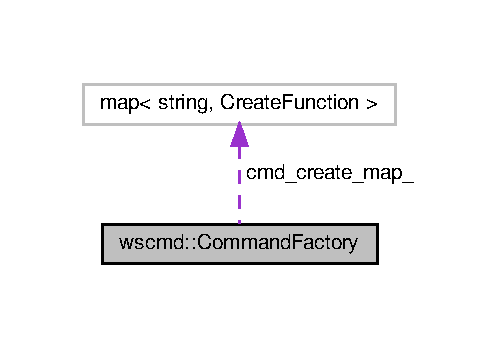
\includegraphics[width=239pt]{classwscmd_1_1CommandFactory__coll__graph}
\end{center}
\end{figure}
\subsection*{Public Types}
\begin{DoxyCompactItemize}
\item 
\mbox{\Hypertarget{classwscmd_1_1CommandFactory_ab6367255c34f4fd923576469acd58c56}\label{classwscmd_1_1CommandFactory_ab6367255c34f4fd923576469acd58c56}} 
using {\bfseries Create\+Function} = Cmd\+Ptr($\ast$)(vector$<$ string $>$ \&\&cmdpara)
\end{DoxyCompactItemize}
\subsection*{Static Public Member Functions}
\begin{DoxyCompactItemize}
\item 
static Cmd\+Ptr \hyperlink{classwscmd_1_1CommandFactory_a3a2ff622076f7ed51fa44de220f61276}{Create\+Cmd} (const string \&cmd\+\_\+string)
\begin{DoxyCompactList}\small\item\em create a command according to the given {\ttfamily name} \end{DoxyCompactList}\item 
static bool \hyperlink{classwscmd_1_1CommandFactory_a3d750b11a80519e15f7e2efbc1f60528}{Register} (const string \&cmd\+\_\+name, Create\+Function \&\&create\+\_\+func)
\begin{DoxyCompactList}\small\item\em Register a command, every command should call this function before program starts. \end{DoxyCompactList}\end{DoxyCompactItemize}
\subsection*{Static Public Attributes}
\begin{DoxyCompactItemize}
\item 
\mbox{\Hypertarget{classwscmd_1_1CommandFactory_a036760d988f21733db305c1777cb08a3}\label{classwscmd_1_1CommandFactory_a036760d988f21733db305c1777cb08a3}} 
static map$<$ string, Create\+Function $>$ {\bfseries cmd\+\_\+create\+\_\+map\+\_\+}
\end{DoxyCompactItemize}


\subsection{Detailed Description}
factory to create command, user of command should use this factory instead of direct new/delete 

\subsection{Member Function Documentation}
\mbox{\Hypertarget{classwscmd_1_1CommandFactory_a3a2ff622076f7ed51fa44de220f61276}\label{classwscmd_1_1CommandFactory_a3a2ff622076f7ed51fa44de220f61276}} 
\index{wscmd\+::\+Command\+Factory@{wscmd\+::\+Command\+Factory}!Create\+Cmd@{Create\+Cmd}}
\index{Create\+Cmd@{Create\+Cmd}!wscmd\+::\+Command\+Factory@{wscmd\+::\+Command\+Factory}}
\subsubsection{\texorpdfstring{Create\+Cmd()}{CreateCmd()}}
{\footnotesize\ttfamily Cmd\+Ptr wscmd\+::\+Command\+Factory\+::\+Create\+Cmd (\begin{DoxyParamCaption}\item[{const string \&}]{cmd\+\_\+string }\end{DoxyParamCaption})\hspace{0.3cm}{\ttfamily [static]}}



create a command according to the given {\ttfamily name} 


\begin{DoxyParams}{Parameters}
{\em cmd\+\_\+name} & command name \\
\hline
{\em para} & command parameters\\
\hline
\end{DoxyParams}
\begin{DoxyReturn}{Returns}
nullptr on failure 
\end{DoxyReturn}
\mbox{\Hypertarget{classwscmd_1_1CommandFactory_a3d750b11a80519e15f7e2efbc1f60528}\label{classwscmd_1_1CommandFactory_a3d750b11a80519e15f7e2efbc1f60528}} 
\index{wscmd\+::\+Command\+Factory@{wscmd\+::\+Command\+Factory}!Register@{Register}}
\index{Register@{Register}!wscmd\+::\+Command\+Factory@{wscmd\+::\+Command\+Factory}}
\subsubsection{\texorpdfstring{Register()}{Register()}}
{\footnotesize\ttfamily bool wscmd\+::\+Command\+Factory\+::\+Register (\begin{DoxyParamCaption}\item[{const string \&}]{cmd\+\_\+name,  }\item[{Create\+Function \&\&}]{create\+\_\+func }\end{DoxyParamCaption})\hspace{0.3cm}{\ttfamily [static]}}



Register a command, every command should call this function before program starts. 


\begin{DoxyParams}{Parameters}
{\em cmd\+\_\+name} & name of the command, must be unique in a process space \\
\hline
{\em create\+\_\+func} & function to create a cmd \\
\hline
\end{DoxyParams}
\begin{DoxyReturn}{Returns}
true if succeed, else false 
\end{DoxyReturn}


The documentation for this class was generated from the following files\+:\begin{DoxyCompactItemize}
\item 
src/websocket\+\_\+server/cmd\+\_\+factory.\+h\item 
src/websocket\+\_\+server/cmd\+\_\+factory.\+cpp\end{DoxyCompactItemize}

\hypertarget{classadpc_1_1Config}{}\section{adpc\+:\+:Config Class Reference}
\label{classadpc_1_1Config}\index{adpc\+::\+Config@{adpc\+::\+Config}}


The \hyperlink{classadpc_1_1Config}{Config} class.  




{\ttfamily \#include $<$config.\+h$>$}

\subsection*{Public Member Functions}
\begin{DoxyCompactItemize}
\item 
\mbox{\Hypertarget{classadpc_1_1Config_a2a68eb461b5842d2a36fbcc5efddaab2}\label{classadpc_1_1Config_a2a68eb461b5842d2a36fbcc5efddaab2}} 
bool {\bfseries Load} ()
\end{DoxyCompactItemize}
\textbf{ }\par
\begin{DoxyCompactItemize}
\item 
string \hyperlink{classadpc_1_1Config_aeb4893a500149d3ae44614767e496132}{Get\+String} (const string \&section, const string \&key)
\begin{DoxyCompactList}\small\item\em getter \end{DoxyCompactList}\item 
int64\+\_\+t \hyperlink{classadpc_1_1Config_a8153d1c7be58fa8ce1a6c768bd65ea94}{Get\+Int} (const string \&section, const string \&key)
\begin{DoxyCompactList}\small\item\em Get integer value. \end{DoxyCompactList}\item 
bool \hyperlink{classadpc_1_1Config_a42a33471c732cd4960e5fb3e00e3b433}{Get\+Bool} (const string \&section, const string \&key)
\begin{DoxyCompactList}\small\item\em Get boolean value. \end{DoxyCompactList}\end{DoxyCompactItemize}



\subsection{Detailed Description}
The \hyperlink{classadpc_1_1Config}{Config} class. 

read config file 

\subsection{Member Function Documentation}
\mbox{\Hypertarget{classadpc_1_1Config_a42a33471c732cd4960e5fb3e00e3b433}\label{classadpc_1_1Config_a42a33471c732cd4960e5fb3e00e3b433}} 
\index{adpc\+::\+Config@{adpc\+::\+Config}!Get\+Bool@{Get\+Bool}}
\index{Get\+Bool@{Get\+Bool}!adpc\+::\+Config@{adpc\+::\+Config}}
\subsubsection{\texorpdfstring{Get\+Bool()}{GetBool()}}
{\footnotesize\ttfamily bool adpc\+::\+Config\+::\+Get\+Bool (\begin{DoxyParamCaption}\item[{const string \&}]{section,  }\item[{const string \&}]{key }\end{DoxyParamCaption})}



Get boolean value. 


\begin{DoxyParams}{Parameters}
{\em section} & section name \\
\hline
{\em key} & key name \\
\hline
\end{DoxyParams}
\begin{DoxyReturn}{Returns}
return value or {\ttfamily false} if not found 
\end{DoxyReturn}
\mbox{\Hypertarget{classadpc_1_1Config_a8153d1c7be58fa8ce1a6c768bd65ea94}\label{classadpc_1_1Config_a8153d1c7be58fa8ce1a6c768bd65ea94}} 
\index{adpc\+::\+Config@{adpc\+::\+Config}!Get\+Int@{Get\+Int}}
\index{Get\+Int@{Get\+Int}!adpc\+::\+Config@{adpc\+::\+Config}}
\subsubsection{\texorpdfstring{Get\+Int()}{GetInt()}}
{\footnotesize\ttfamily int64\+\_\+t adpc\+::\+Config\+::\+Get\+Int (\begin{DoxyParamCaption}\item[{const string \&}]{section,  }\item[{const string \&}]{key }\end{DoxyParamCaption})}



Get integer value. 


\begin{DoxyParams}{Parameters}
{\em section} & section name \\
\hline
{\em key} & key name \\
\hline
\end{DoxyParams}
\begin{DoxyReturn}{Returns}
return value or {\ttfamily 0} if not found 
\end{DoxyReturn}
\mbox{\Hypertarget{classadpc_1_1Config_aeb4893a500149d3ae44614767e496132}\label{classadpc_1_1Config_aeb4893a500149d3ae44614767e496132}} 
\index{adpc\+::\+Config@{adpc\+::\+Config}!Get\+String@{Get\+String}}
\index{Get\+String@{Get\+String}!adpc\+::\+Config@{adpc\+::\+Config}}
\subsubsection{\texorpdfstring{Get\+String()}{GetString()}}
{\footnotesize\ttfamily string adpc\+::\+Config\+::\+Get\+String (\begin{DoxyParamCaption}\item[{const string \&}]{section,  }\item[{const string \&}]{key }\end{DoxyParamCaption})}



getter 

get string value 
\begin{DoxyParams}{Parameters}
{\em section} & section name \\
\hline
{\em key} & key name \\
\hline
\end{DoxyParams}
\begin{DoxyReturn}{Returns}
return value or empty string if not found 
\end{DoxyReturn}


The documentation for this class was generated from the following files\+:\begin{DoxyCompactItemize}
\item 
src/config/config.\+h\item 
src/config/config.\+cpp\end{DoxyCompactItemize}

\hypertarget{classwscmd_1_1ICommand}{}\section{wscmd\+:\+:I\+Command Class Reference}
\label{classwscmd_1_1ICommand}\index{wscmd\+::\+I\+Command@{wscmd\+::\+I\+Command}}


Commannd interface.  




{\ttfamily \#include $<$command.\+h$>$}



Inheritance diagram for wscmd\+:\+:I\+Command\+:\nopagebreak
\begin{figure}[H]
\begin{center}
\leavevmode
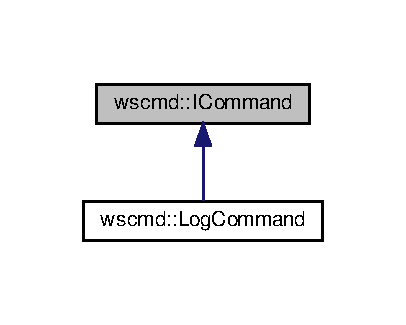
\includegraphics[width=195pt]{classwscmd_1_1ICommand__inherit__graph}
\end{center}
\end{figure}


Collaboration diagram for wscmd\+:\+:I\+Command\+:\nopagebreak
\begin{figure}[H]
\begin{center}
\leavevmode
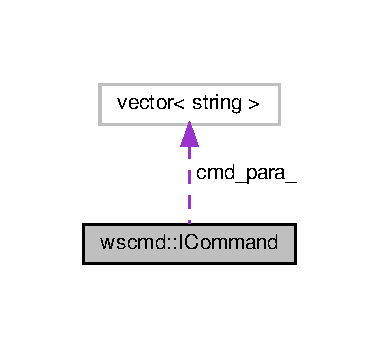
\includegraphics[width=183pt]{classwscmd_1_1ICommand__coll__graph}
\end{center}
\end{figure}
\subsection*{Public Member Functions}
\begin{DoxyCompactItemize}
\item 
\mbox{\Hypertarget{classwscmd_1_1ICommand_ab4768937ccb18cc24d8da7ad91da442a}\label{classwscmd_1_1ICommand_ab4768937ccb18cc24d8da7ad91da442a}} 
{\bfseries I\+Command} (vector$<$ string $>$ \&\&cmd\+\_\+para)
\item 
\mbox{\Hypertarget{classwscmd_1_1ICommand_a9f4adb20beb9c577e1da6a8ef9a4ca43}\label{classwscmd_1_1ICommand_a9f4adb20beb9c577e1da6a8ef9a4ca43}} 
virtual string \hyperlink{classwscmd_1_1ICommand_a9f4adb20beb9c577e1da6a8ef9a4ca43}{Execute} ()=0
\begin{DoxyCompactList}\small\item\em Execute command. \end{DoxyCompactList}\item 
virtual const string \& \hyperlink{classwscmd_1_1ICommand_a1a9fdc32265fa902cb5f3ab153386a9e}{Name} ()=0
\begin{DoxyCompactList}\small\item\em Name of the command, must be unique in the whole program. \end{DoxyCompactList}\end{DoxyCompactItemize}
\subsection*{Protected Attributes}
\begin{DoxyCompactItemize}
\item 
\mbox{\Hypertarget{classwscmd_1_1ICommand_ad8ebb0beab8997eebf9538d2bb9bb9dd}\label{classwscmd_1_1ICommand_ad8ebb0beab8997eebf9538d2bb9bb9dd}} 
vector$<$ string $>$ {\bfseries cmd\+\_\+para\+\_\+}
\item 
\mbox{\Hypertarget{classwscmd_1_1ICommand_a82221aa31e2f2c1ab2b5fdaf082c4faa}\label{classwscmd_1_1ICommand_a82221aa31e2f2c1ab2b5fdaf082c4faa}} 
int {\bfseries cmd\+\_\+argc\+\_\+} \{0\}
\item 
\mbox{\Hypertarget{classwscmd_1_1ICommand_ab18e734b8f8ff025caa26bd441580243}\label{classwscmd_1_1ICommand_ab18e734b8f8ff025caa26bd441580243}} 
char $\ast$$\ast$ {\bfseries cmd\+\_\+argv\+\_\+} \{nullptr\}
\end{DoxyCompactItemize}


\subsection{Detailed Description}
Commannd interface. 

\subsection{Member Function Documentation}
\mbox{\Hypertarget{classwscmd_1_1ICommand_a1a9fdc32265fa902cb5f3ab153386a9e}\label{classwscmd_1_1ICommand_a1a9fdc32265fa902cb5f3ab153386a9e}} 
\index{wscmd\+::\+I\+Command@{wscmd\+::\+I\+Command}!Name@{Name}}
\index{Name@{Name}!wscmd\+::\+I\+Command@{wscmd\+::\+I\+Command}}
\subsubsection{\texorpdfstring{Name()}{Name()}}
{\footnotesize\ttfamily virtual const string\& wscmd\+::\+I\+Command\+::\+Name (\begin{DoxyParamCaption}{ }\end{DoxyParamCaption})\hspace{0.3cm}{\ttfamily [pure virtual]}}



Name of the command, must be unique in the whole program. 

\begin{DoxyReturn}{Returns}

\end{DoxyReturn}


Implemented in \hyperlink{classwscmd_1_1LogCommand_a465f14b51110d3f0a7d5fe873bafd857}{wscmd\+::\+Log\+Command}.



The documentation for this class was generated from the following files\+:\begin{DoxyCompactItemize}
\item 
src/websocket\+\_\+server/command.\+h\item 
src/websocket\+\_\+server/command.\+cpp\end{DoxyCompactItemize}

\hypertarget{classadpc_1_1Log}{}\section{adpc\+:\+:Log Class Reference}
\label{classadpc_1_1Log}\index{adpc\+::\+Log@{adpc\+::\+Log}}


The log class for vincent.  




{\ttfamily \#include $<$log.\+h$>$}

\subsection*{Public Member Functions}
\begin{DoxyCompactItemize}
\item 
void \hyperlink{classadpc_1_1Log_a2e8bf1e2c8ac8381be9022df60530f87}{Set\+Level} (const string \&module\+\_\+name, const Log\+Sink\+Type type, const \hyperlink{log__config_8h_a172986fa5f658c5fe0b42bd954e9e133}{Log\+Level} level)
\item 
\mbox{\Hypertarget{classadpc_1_1Log_ae9c832f1a8d5f684308f5ef95d53cf36}\label{classadpc_1_1Log_ae9c832f1a8d5f684308f5ef95d53cf36}} 
void {\bfseries Enable} (const string \&module\+\_\+name, const Log\+Sink\+Type type, const bool enable)
\item 
\mbox{\Hypertarget{classadpc_1_1Log_a599ccdccf8a85ae3779a8f587424cea8}\label{classadpc_1_1Log_a599ccdccf8a85ae3779a8f587424cea8}} 
void {\bfseries Add\+Module} (string \&\&module\+\_\+name, const \hyperlink{log__config_8h_a172986fa5f658c5fe0b42bd954e9e133}{Log\+Level} level=Log\+Level\+::warn, const bool terminal=true, const bool daily\+\_\+file=true)
\end{DoxyCompactItemize}
\textbf{ }\par
\begin{DoxyCompactItemize}
\item 
{\footnotesize template$<$typename... Args$>$ }\\void \hyperlink{classadpc_1_1Log_ae3e21b4038776f15d0b5ebdfebc41f57}{log} (\hyperlink{log__config_8h_a172986fa5f658c5fe0b42bd954e9e133}{Log\+Level} lvl, const char $\ast$fmt, const Args \&... args)
\end{DoxyCompactItemize}

\subsection*{Static Public Member Functions}
\begin{DoxyCompactItemize}
\item 
static void \hyperlink{classadpc_1_1Log_a41b80ba97a00d128777d22f369bc791f}{Init\+Path} ()
\begin{DoxyCompactList}\small\item\em create directory if not exist \end{DoxyCompactList}\end{DoxyCompactItemize}
\subsection*{Friends}
\begin{DoxyCompactItemize}
\item 
\mbox{\Hypertarget{classadpc_1_1Log_a0e7b4c16064e3789d935b1b3523d78c7}\label{classadpc_1_1Log_a0e7b4c16064e3789d935b1b3523d78c7}} 
class {\bfseries adpctl\+::\+Singleton$<$ Log $>$}
\end{DoxyCompactItemize}


\subsection{Detailed Description}
The log class for vincent. 

contains one daily file and a color terminal

destination path of log is ./log/ 

\subsection{Member Function Documentation}
\mbox{\Hypertarget{classadpc_1_1Log_a41b80ba97a00d128777d22f369bc791f}\label{classadpc_1_1Log_a41b80ba97a00d128777d22f369bc791f}} 
\index{adpc\+::\+Log@{adpc\+::\+Log}!Init\+Path@{Init\+Path}}
\index{Init\+Path@{Init\+Path}!adpc\+::\+Log@{adpc\+::\+Log}}
\subsubsection{\texorpdfstring{Init\+Path()}{InitPath()}}
{\footnotesize\ttfamily void adpc\+::\+Log\+::\+Init\+Path (\begin{DoxyParamCaption}{ }\end{DoxyParamCaption})\hspace{0.3cm}{\ttfamily [static]}}



create directory if not exist 

\begin{DoxyWarning}{Warning}
call this function before any call to log, or you may crash your program
\end{DoxyWarning}
this funtion is guaranteed to be executed once enen if you call multiple times from multi-\/threads \mbox{\Hypertarget{classadpc_1_1Log_ae3e21b4038776f15d0b5ebdfebc41f57}\label{classadpc_1_1Log_ae3e21b4038776f15d0b5ebdfebc41f57}} 
\index{adpc\+::\+Log@{adpc\+::\+Log}!log@{log}}
\index{log@{log}!adpc\+::\+Log@{adpc\+::\+Log}}
\subsubsection{\texorpdfstring{log()}{log()}}
{\footnotesize\ttfamily template$<$typename... Args$>$ \\
void adpc\+::\+Log\+::log (\begin{DoxyParamCaption}\item[{\hyperlink{log__config_8h_a172986fa5f658c5fe0b42bd954e9e133}{Log\+Level}}]{lvl,  }\item[{const char $\ast$}]{fmt,  }\item[{const Args \&...}]{args }\end{DoxyParamCaption})\hspace{0.3cm}{\ttfamily [inline]}}

general log function \mbox{\Hypertarget{classadpc_1_1Log_a2e8bf1e2c8ac8381be9022df60530f87}\label{classadpc_1_1Log_a2e8bf1e2c8ac8381be9022df60530f87}} 
\index{adpc\+::\+Log@{adpc\+::\+Log}!Set\+Level@{Set\+Level}}
\index{Set\+Level@{Set\+Level}!adpc\+::\+Log@{adpc\+::\+Log}}
\subsubsection{\texorpdfstring{Set\+Level()}{SetLevel()}}
{\footnotesize\ttfamily void adpc\+::\+Log\+::\+Set\+Level (\begin{DoxyParamCaption}\item[{const string \&}]{module\+\_\+name,  }\item[{const Log\+Sink\+Type}]{type,  }\item[{const \hyperlink{log__config_8h_a172986fa5f658c5fe0b42bd954e9e133}{Log\+Level}}]{level }\end{DoxyParamCaption})\hspace{0.3cm}{\ttfamily [inline]}}



The documentation for this class was generated from the following files\+:\begin{DoxyCompactItemize}
\item 
src/log/log.\+h\item 
src/log/log.\+cpp\end{DoxyCompactItemize}

\hypertarget{classwscmd_1_1LogCommand}{}\section{wscmd\+:\+:Log\+Command Class Reference}
\label{classwscmd_1_1LogCommand}\index{wscmd\+::\+Log\+Command@{wscmd\+::\+Log\+Command}}


Inheritance diagram for wscmd\+:\+:Log\+Command\+:\nopagebreak
\begin{figure}[H]
\begin{center}
\leavevmode
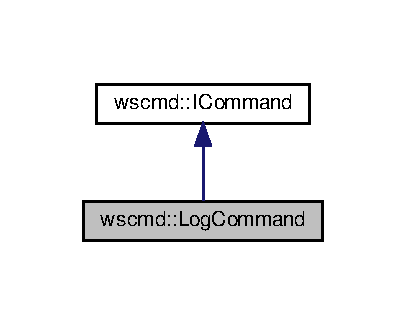
\includegraphics[width=195pt]{classwscmd_1_1LogCommand__inherit__graph}
\end{center}
\end{figure}


Collaboration diagram for wscmd\+:\+:Log\+Command\+:\nopagebreak
\begin{figure}[H]
\begin{center}
\leavevmode
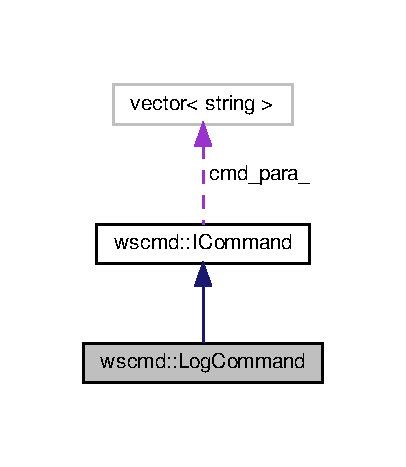
\includegraphics[width=195pt]{classwscmd_1_1LogCommand__coll__graph}
\end{center}
\end{figure}
\subsection*{Public Member Functions}
\begin{DoxyCompactItemize}
\item 
\mbox{\Hypertarget{classwscmd_1_1LogCommand_a805597e0d733814ff3238bcb99c8041a}\label{classwscmd_1_1LogCommand_a805597e0d733814ff3238bcb99c8041a}} 
{\bfseries Log\+Command} (vector$<$ string $>$ \&\&cmd\+\_\+para)
\item 
\mbox{\Hypertarget{classwscmd_1_1LogCommand_a9ef233e03aa8736cd9578ba015161efb}\label{classwscmd_1_1LogCommand_a9ef233e03aa8736cd9578ba015161efb}} 
string \hyperlink{classwscmd_1_1LogCommand_a9ef233e03aa8736cd9578ba015161efb}{Execute} () override
\begin{DoxyCompactList}\small\item\em Execute command. \end{DoxyCompactList}\item 
const string \& \hyperlink{classwscmd_1_1LogCommand_a465f14b51110d3f0a7d5fe873bafd857}{Name} () override
\begin{DoxyCompactList}\small\item\em Name of the command, must be unique in the whole program. \end{DoxyCompactList}\end{DoxyCompactItemize}
\subsection*{Static Public Member Functions}
\begin{DoxyCompactItemize}
\item 
\mbox{\Hypertarget{classwscmd_1_1LogCommand_a027391b953d2e1aa9a7655b058639f80}\label{classwscmd_1_1LogCommand_a027391b953d2e1aa9a7655b058639f80}} 
static Cmd\+Ptr {\bfseries Create} (vector$<$ string $>$ \&\&cmd\+\_\+para)
\end{DoxyCompactItemize}
\subsection*{Static Public Attributes}
\begin{DoxyCompactItemize}
\item 
\mbox{\Hypertarget{classwscmd_1_1LogCommand_a6f599e38cd04f3c29b2b4e9f9ada8ce4}\label{classwscmd_1_1LogCommand_a6f599e38cd04f3c29b2b4e9f9ada8ce4}} 
static bool {\bfseries is\+\_\+registered\+\_\+} = \hyperlink{classwscmd_1_1CommandFactory_a3d750b11a80519e15f7e2efbc1f60528}{Command\+Factory\+::\+Register}(\char`\"{}log\char`\"{}, Log\+Command\+::\+Create)
\end{DoxyCompactItemize}
\subsection*{Additional Inherited Members}


\subsection{Member Function Documentation}
\mbox{\Hypertarget{classwscmd_1_1LogCommand_a465f14b51110d3f0a7d5fe873bafd857}\label{classwscmd_1_1LogCommand_a465f14b51110d3f0a7d5fe873bafd857}} 
\index{wscmd\+::\+Log\+Command@{wscmd\+::\+Log\+Command}!Name@{Name}}
\index{Name@{Name}!wscmd\+::\+Log\+Command@{wscmd\+::\+Log\+Command}}
\subsubsection{\texorpdfstring{Name()}{Name()}}
{\footnotesize\ttfamily const string \& wscmd\+::\+Log\+Command\+::\+Name (\begin{DoxyParamCaption}{ }\end{DoxyParamCaption})\hspace{0.3cm}{\ttfamily [override]}, {\ttfamily [virtual]}}



Name of the command, must be unique in the whole program. 

\begin{DoxyReturn}{Returns}

\end{DoxyReturn}


Implements \hyperlink{classwscmd_1_1ICommand_a1a9fdc32265fa902cb5f3ab153386a9e}{wscmd\+::\+I\+Command}.



The documentation for this class was generated from the following files\+:\begin{DoxyCompactItemize}
\item 
src/websocket\+\_\+server/log\+\_\+cmd.\+h\item 
src/websocket\+\_\+server/log\+\_\+cmd.\+cpp\end{DoxyCompactItemize}

\hypertarget{classadpc_1_1LogConfiguration}{}\section{adpc\+:\+:Log\+Configuration Class Reference}
\label{classadpc_1_1LogConfiguration}\index{adpc\+::\+Log\+Configuration@{adpc\+::\+Log\+Configuration}}
\subsection*{Friends}
\begin{DoxyCompactItemize}
\item 
\mbox{\Hypertarget{classadpc_1_1LogConfiguration_acd1b2a0733103b7bbeb76b467ea85446}\label{classadpc_1_1LogConfiguration_acd1b2a0733103b7bbeb76b467ea85446}} 
class {\bfseries Log}
\end{DoxyCompactItemize}


The documentation for this class was generated from the following file\+:\begin{DoxyCompactItemize}
\item 
src/log/\hyperlink{log__config_8h}{log\+\_\+config.\+h}\end{DoxyCompactItemize}

\hypertarget{classMutexLock}{}\section{Mutex\+Lock Class Reference}
\label{classMutexLock}\index{Mutex\+Lock@{Mutex\+Lock}}
\subsection*{Public Member Functions}
\begin{DoxyCompactItemize}
\item 
\mbox{\Hypertarget{classMutexLock_ac2b61ce467a009859472ca688e78a3b1}\label{classMutexLock_ac2b61ce467a009859472ca688e78a3b1}} 
int {\bfseries lock} ()
\item 
\mbox{\Hypertarget{classMutexLock_acfcff8cc8d51ad233d341844e4feb4a6}\label{classMutexLock_acfcff8cc8d51ad233d341844e4feb4a6}} 
int {\bfseries unlock} ()
\end{DoxyCompactItemize}


The documentation for this class was generated from the following files\+:\begin{DoxyCompactItemize}
\item 
src/http/manager\+\_\+lock.\+h\item 
src/http/manager\+\_\+lock.\+cpp\end{DoxyCompactItemize}

\hypertarget{classadpctl_1_1Singleton}{}\section{adpctl\+:\+:Singleton$<$ T $>$ Class Template Reference}
\label{classadpctl_1_1Singleton}\index{adpctl\+::\+Singleton$<$ T $>$@{adpctl\+::\+Singleton$<$ T $>$}}
\subsection*{Static Public Member Functions}
\begin{DoxyCompactItemize}
\item 
\mbox{\Hypertarget{classadpctl_1_1Singleton_af082cd0385253eb507206f2c8b85a398}\label{classadpctl_1_1Singleton_af082cd0385253eb507206f2c8b85a398}} 
static Type \& {\bfseries Get\+Instance} ()
\end{DoxyCompactItemize}


The documentation for this class was generated from the following file\+:\begin{DoxyCompactItemize}
\item 
src/adpctl/singleton.\+h\end{DoxyCompactItemize}

\hypertarget{classWSServer}{}\section{W\+S\+Server Class Reference}
\label{classWSServer}\index{W\+S\+Server@{W\+S\+Server}}


The documentation for this class was generated from the following files\+:\begin{DoxyCompactItemize}
\item 
src/websocket\+\_\+server/websocket\+\_\+server.\+h\item 
src/websocket\+\_\+server/websocket\+\_\+server.\+cpp\end{DoxyCompactItemize}

\chapter{File Documentation}
\hypertarget{main_8cpp}{}\section{src/app/main.cpp File Reference}
\label{main_8cpp}\index{src/app/main.\+cpp@{src/app/main.\+cpp}}
{\ttfamily \#include $<$iostream$>$}\newline
{\ttfamily \#include $<$string$>$}\newline
Include dependency graph for main.\+cpp\+:\nopagebreak
\begin{figure}[H]
\begin{center}
\leavevmode
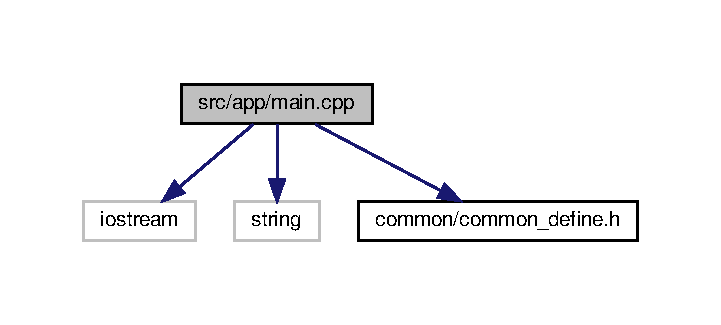
\includegraphics[width=194pt]{main_8cpp__incl}
\end{center}
\end{figure}
\subsection*{Functions}
\begin{DoxyCompactItemize}
\item 
\mbox{\Hypertarget{main_8cpp_a3c04138a5bfe5d72780bb7e82a18e627}\label{main_8cpp_a3c04138a5bfe5d72780bb7e82a18e627}} 
int {\bfseries main} (int argc, char $\ast$$\ast$argv)
\end{DoxyCompactItemize}


\subsection{Detailed Description}
\begin{DoxyAuthor}{Author}
your name (\href{mailto:you@domain.com}{\tt you@domain.\+com}) 
\end{DoxyAuthor}
\begin{DoxyVersion}{Version}
0.\+1 
\end{DoxyVersion}
\begin{DoxyDate}{Date}
2019-\/05-\/01
\end{DoxyDate}
\begin{DoxyCopyright}{Copyright}
Copyright (c) 2019 
\end{DoxyCopyright}

\hypertarget{common__define_8h}{}\section{src/common/common\+\_\+define.h File Reference}
\label{common__define_8h}\index{src/common/common\+\_\+define.\+h@{src/common/common\+\_\+define.\+h}}


common define for vincent project of Advanced Data Processing Company(\+A\+D\+P\+C) many macros has A\+D\+PC prefix  


This graph shows which files directly or indirectly include this file\+:\nopagebreak
\begin{figure}[H]
\begin{center}
\leavevmode
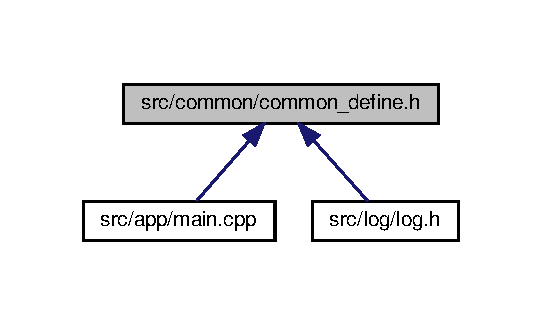
\includegraphics[width=260pt]{common__define_8h__dep__incl}
\end{center}
\end{figure}
\subsection*{Macros}
\begin{DoxyCompactItemize}
\item 
\mbox{\Hypertarget{common__define_8h_a1ebba11cb2b65ac03b4a160b784a4cf5}\label{common__define_8h_a1ebba11cb2b65ac03b4a160b784a4cf5}} 
\#define \hyperlink{common__define_8h_a1ebba11cb2b65ac03b4a160b784a4cf5}{A\+D\+P\+C\+\_\+\+U\+N\+U\+S\+ED}
\begin{DoxyCompactList}\small\item\em Unused mark, unused varable must be marked with this tag or will trigger an error in compilling. \end{DoxyCompactList}\item 
\mbox{\Hypertarget{common__define_8h_ae35e82ea2c24a982c3a3371856adb181}\label{common__define_8h_ae35e82ea2c24a982c3a3371856adb181}} 
\#define \hyperlink{common__define_8h_ae35e82ea2c24a982c3a3371856adb181}{A\+D\+P\+C\+\_\+\+D\+E\+P\+R\+E\+C\+A\+T\+ED}(msg)
\begin{DoxyCompactList}\small\item\em deprecated mark, unsed api should be marked by this for better documentation if cpp compiler is c+=14 or newer, standard {\ttfamily deprecated} is used else gnu extension is used \end{DoxyCompactList}\item 
\mbox{\Hypertarget{common__define_8h_a88dfb71ec507f8d8515fd194fbe67ec4}\label{common__define_8h_a88dfb71ec507f8d8515fd194fbe67ec4}} 
\#define \hyperlink{common__define_8h_a88dfb71ec507f8d8515fd194fbe67ec4}{A\+D\+P\+C\+\_\+\+L\+I\+K\+E\+LY}(exp)
\begin{DoxyCompactList}\small\item\em likey path \end{DoxyCompactList}\item 
\mbox{\Hypertarget{common__define_8h_a2308a86bb0e477c6bd4ee0f6571e29ca}\label{common__define_8h_a2308a86bb0e477c6bd4ee0f6571e29ca}} 
\#define \hyperlink{common__define_8h_a2308a86bb0e477c6bd4ee0f6571e29ca}{A\+D\+P\+C\+\_\+\+U\+N\+L\+I\+K\+E\+LY}(exp)
\begin{DoxyCompactList}\small\item\em unlikey path \end{DoxyCompactList}\item 
\mbox{\Hypertarget{common__define_8h_aa78f1a5365c33985492e85eea9daa0b6}\label{common__define_8h_aa78f1a5365c33985492e85eea9daa0b6}} 
\#define \hyperlink{common__define_8h_aa78f1a5365c33985492e85eea9daa0b6}{A\+D\+P\+C\+\_\+\+A\+S\+S\+E\+RT}(condition,  msg)
\begin{DoxyCompactList}\small\item\em assertation \end{DoxyCompactList}\end{DoxyCompactItemize}


\subsection{Detailed Description}
common define for vincent project of Advanced Data Processing Company(\+A\+D\+P\+C) many macros has A\+D\+PC prefix 

\begin{DoxyAuthor}{Author}
tonghao.\+yuan (\href{mailto:michael.19@163.com}{\tt michael.\+19@163.\+com}) 
\end{DoxyAuthor}
\begin{DoxyVersion}{Version}
0.\+1 
\end{DoxyVersion}
\begin{DoxyDate}{Date}
2019-\/05-\/04
\end{DoxyDate}
\begin{DoxyCopyright}{Copyright}
Copyright (c) 2019 
\end{DoxyCopyright}

\hypertarget{os_8h}{}\section{src/common/os.h File Reference}
\label{os_8h}\index{src/common/os.\+h@{src/common/os.\+h}}


os relative convinient functions  


{\ttfamily \#include $<$string$>$}\newline
Include dependency graph for os.\+h\+:\nopagebreak
\begin{figure}[H]
\begin{center}
\leavevmode
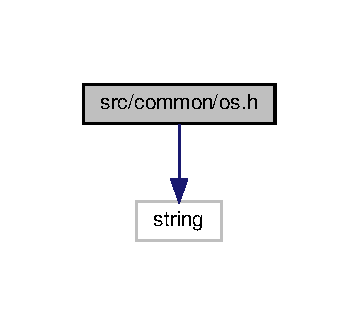
\includegraphics[width=172pt]{os_8h__incl}
\end{center}
\end{figure}
\subsection*{Functions}
\begin{DoxyCompactItemize}
\item 
bool {\bfseries adpc\+::os\+::\+File\+Exists} (const string \&file\+\_\+full\+\_\+path)
\begin{DoxyCompactList}\small\item\em check if a file exists. \end{DoxyCompactList}\item 
\mbox{\Hypertarget{os_8cpp_a1e8590fbb8a2c3da313cdfffe2a01097}\label{os_8cpp_a1e8590fbb8a2c3da313cdfffe2a01097}} 
string {\bfseries adpc\+::os\+::\+Get\+Current\+Directory} ()
\end{DoxyCompactItemize}


\subsection{Detailed Description}
os relative convinient functions 

\begin{DoxyAuthor}{Author}
tonghao.\+yuan (\href{mailto:michael.19@163.com}{\tt michael.\+19@163.\+com}) 
\end{DoxyAuthor}
\begin{DoxyVersion}{Version}
0.\+1 
\end{DoxyVersion}
\begin{DoxyDate}{Date}
2019-\/05-\/12
\end{DoxyDate}
\begin{DoxyCopyright}{Copyright}
Copyright (c) 2019 
\end{DoxyCopyright}


\subsection{Function Documentation}
\mbox{\Hypertarget{os_8cpp_file_a16e4cbb08e5d085a2581999342b1212a}\label{os_8cpp_file_a16e4cbb08e5d085a2581999342b1212a}} 
\index{os.\+h@{os.\+h}!File\+Exists@{File\+Exists}}
\index{File\+Exists@{File\+Exists}!os.\+h@{os.\+h}}
\subsubsection{\texorpdfstring{File\+Exists()}{FileExists()}}
{\footnotesize\ttfamily bool adpc\+::os\+::\+File\+Exists (\begin{DoxyParamCaption}\item[{const string \&}]{file\+\_\+full\+\_\+path }\end{DoxyParamCaption})}



check if a file exists. 


\begin{DoxyParams}{Parameters}
{\em file\+\_\+full\+\_\+path} & full path to the file, relative or absolute path both ok \\
\hline
\end{DoxyParams}
\begin{DoxyReturn}{Returns}
true for exists, false for not 
\end{DoxyReturn}

\hypertarget{log_8h}{}\section{src/log/log.h File Reference}
\label{log_8h}\index{src/log/log.\+h@{src/log/log.\+h}}


log module of vincent  


{\ttfamily \#include \char`\"{}adpctl/singleton.\+h\char`\"{}}\newline
{\ttfamily \#include \char`\"{}common/common\+\_\+define.\+h\char`\"{}}\newline
{\ttfamily \#include \char`\"{}log/log\+\_\+config.\+h\char`\"{}}\newline
{\ttfamily \#include $<$atomic$>$}\newline
{\ttfamily \#include $<$map$>$}\newline
{\ttfamily \#include $<$memory$>$}\newline
{\ttfamily \#include $<$sstream$>$}\newline
{\ttfamily \#include $<$string$>$}\newline
{\ttfamily \#include $<$vector$>$}\newline
{\ttfamily \#include \char`\"{}spdlog/sinks/daily\+\_\+file\+\_\+sink.\+h\char`\"{}}\newline
{\ttfamily \#include \char`\"{}spdlog/sinks/stdout\+\_\+color\+\_\+sinks.\+h\char`\"{}}\newline
{\ttfamily \#include \char`\"{}spdlog/spdlog.\+h\char`\"{}}\newline
Include dependency graph for log.\+h\+:\nopagebreak
\begin{figure}[H]
\begin{center}
\leavevmode
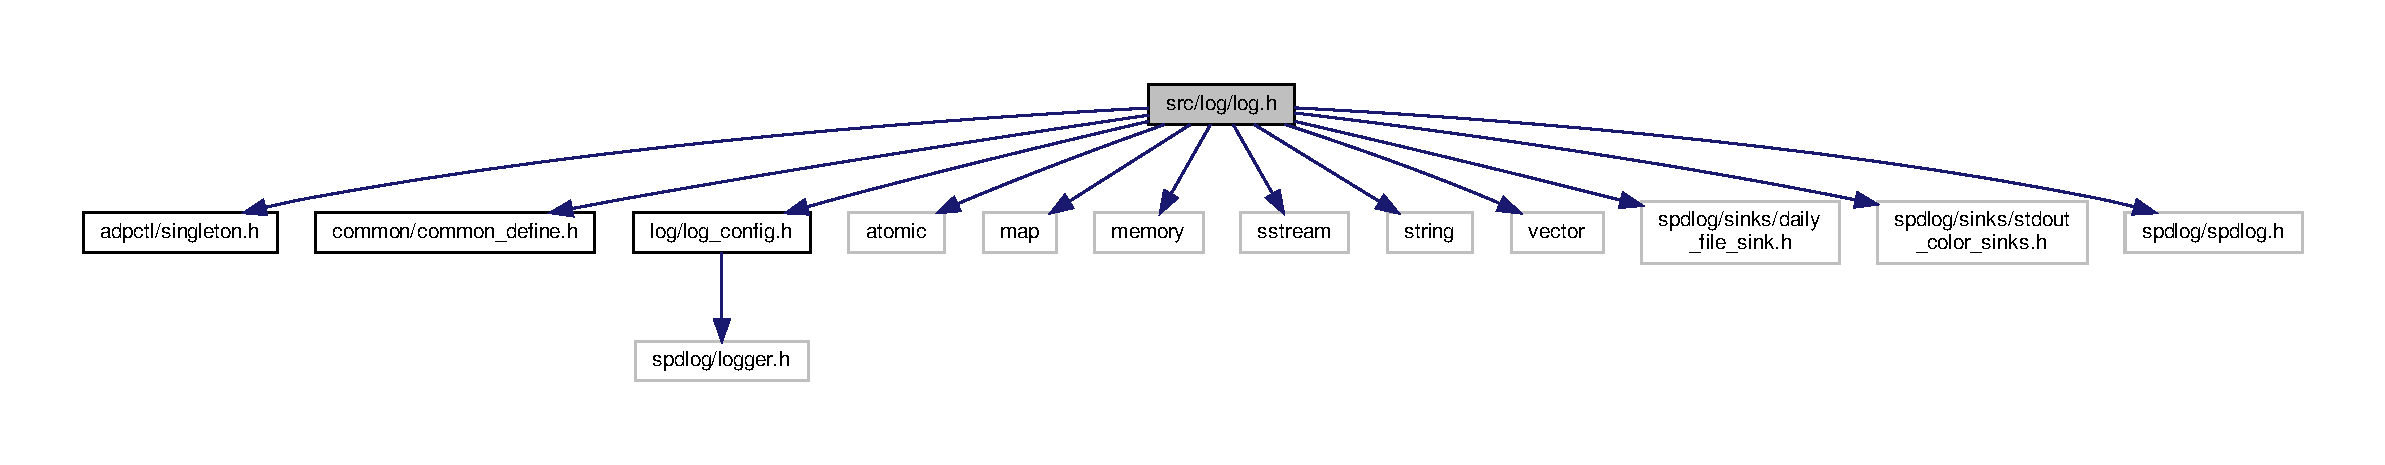
\includegraphics[width=350pt]{log_8h__incl}
\end{center}
\end{figure}
\subsection*{Classes}
\begin{DoxyCompactItemize}
\item 
class \hyperlink{classadpc_1_1Log}{adpc\+::\+Log}
\begin{DoxyCompactList}\small\item\em The log class for vincent. \end{DoxyCompactList}\end{DoxyCompactItemize}
\subsection*{Macros}
\begin{DoxyCompactItemize}
\item 
\#define {\bfseries A\+D\+P\+C\+\_\+\+L\+O\+G\+\_\+\+N\+A\+ME}(lvl)
\item 
\mbox{\Hypertarget{log_8h_a159ca84d25a5487d8e81e4438725df19}\label{log_8h_a159ca84d25a5487d8e81e4438725df19}} 
\#define {\bfseries L\+OG}~\hyperlink{classadpctl_1_1Singleton}{adpctl\+::\+Singleton}$<$\hyperlink{classadpc_1_1Log}{adpc\+::\+Log}$>$\+::Get\+Instance()
\end{DoxyCompactItemize}


\subsection{Detailed Description}
log module of vincent 

\begin{DoxyAuthor}{Author}
tonghao.\+yuan (\href{mailto:michael.19@163.com}{\tt michael.\+19@163.\+com}) This log have multiple front-\/end and multiple back-\/end every module can have its own front-\/end by call 
\end{DoxyAuthor}
\begin{DoxySeeAlso}{See also}
Add\+Module ervey module can have its own log level 
\end{DoxySeeAlso}
\begin{DoxyWarning}{Warning}
placehoder is {\ttfamily \{\}}
\end{DoxyWarning}
\begin{DoxyVersion}{Version}
0.\+1 
\end{DoxyVersion}
\begin{DoxyDate}{Date}
2019-\/05-\/17
\end{DoxyDate}
\begin{DoxyCopyright}{Copyright}
Copyright (c) 2019 
\end{DoxyCopyright}


\subsection{Macro Definition Documentation}
\mbox{\Hypertarget{log_8h_a8a890200ead6b94208877afe7d9b764c}\label{log_8h_a8a890200ead6b94208877afe7d9b764c}} 
\index{log.\+h@{log.\+h}!A\+D\+P\+C\+\_\+\+L\+O\+G\+\_\+\+N\+A\+ME@{A\+D\+P\+C\+\_\+\+L\+O\+G\+\_\+\+N\+A\+ME}}
\index{A\+D\+P\+C\+\_\+\+L\+O\+G\+\_\+\+N\+A\+ME@{A\+D\+P\+C\+\_\+\+L\+O\+G\+\_\+\+N\+A\+ME}!log.\+h@{log.\+h}}
\subsubsection{\texorpdfstring{A\+D\+P\+C\+\_\+\+L\+O\+G\+\_\+\+N\+A\+ME}{ADPC\_LOG\_NAME}}
{\footnotesize\ttfamily \#define A\+D\+P\+C\+\_\+\+L\+O\+G\+\_\+\+N\+A\+ME(\begin{DoxyParamCaption}\item[{}]{lvl }\end{DoxyParamCaption})}

{\bfseries Value\+:}
\begin{DoxyCode}
\textcolor{keyword}{template} <\textcolor{keyword}{typename}... Args>                                                   \(\backslash\)
    void lvl(\textcolor{keywordtype}{size\_t}      module,                                                  \(\backslash\)
             \textcolor{keyword}{const} \textcolor{keywordtype}{char} *file,                                                    \(\backslash\)
             \textcolor{keywordtype}{int}         line,                                                    \(\backslash\)
             \textcolor{keyword}{const} \textcolor{keywordtype}{char} *func,                                                    \(\backslash\)
             \textcolor{keyword}{const} \textcolor{keywordtype}{char} *fmt,                                                     \(\backslash\)
             \textcolor{keyword}{const} Args &... args) \{                                              \(\backslash\)
        assert(module < logs\_.size());                                            \(\backslash\)
        logs\_[module]->log(\{file, line, func\}, spdlog::level::lvl, fmt, args...); \(\backslash\)
    \}
\end{DoxyCode}

\hypertarget{log__config_8h}{}\section{src/log/log\+\_\+config.h File Reference}
\label{log__config_8h}\index{src/log/log\+\_\+config.\+h@{src/log/log\+\_\+config.\+h}}


configuration for log sinks  


{\ttfamily \#include \char`\"{}spdlog/logger.\+h\char`\"{}}\newline
Include dependency graph for log\+\_\+config.\+h\+:\nopagebreak
\begin{figure}[H]
\begin{center}
\leavevmode
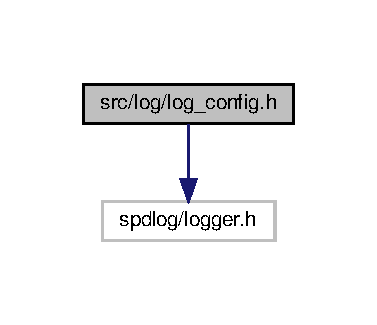
\includegraphics[width=181pt]{log__config_8h__incl}
\end{center}
\end{figure}
This graph shows which files directly or indirectly include this file\+:\nopagebreak
\begin{figure}[H]
\begin{center}
\leavevmode
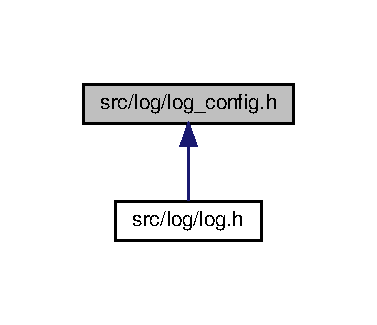
\includegraphics[width=181pt]{log__config_8h__dep__incl}
\end{center}
\end{figure}
\subsection*{Classes}
\begin{DoxyCompactItemize}
\item 
class \hyperlink{classadpc_1_1LogConfiguration}{adpc\+::\+Log\+Configuration}
\end{DoxyCompactItemize}
\subsection*{Enumerations}
\begin{DoxyCompactItemize}
\item 
\mbox{\Hypertarget{log__config_8h_aed0c9a77837fba12dc47392177b41606}\label{log__config_8h_aed0c9a77837fba12dc47392177b41606}} 
enum {\bfseries Log\+Sink\+Type} \{ {\bfseries kdaily\+\_\+file}, 
{\bfseries kterminal}
 \}
\item 
enum \hyperlink{log__config_8h_a172986fa5f658c5fe0b42bd954e9e133}{adpc\+::\+Log\+Level} \{ \newline
{\bfseries ktrace} = S\+P\+D\+L\+O\+G\+\_\+\+L\+E\+V\+E\+L\+\_\+\+T\+R\+A\+CE, 
{\bfseries kdebug} = S\+P\+D\+L\+O\+G\+\_\+\+L\+E\+V\+E\+L\+\_\+\+D\+E\+B\+UG, 
{\bfseries kinfo} = S\+P\+D\+L\+O\+G\+\_\+\+L\+E\+V\+E\+L\+\_\+\+I\+N\+FO, 
{\bfseries kwarn} = S\+P\+D\+L\+O\+G\+\_\+\+L\+E\+V\+E\+L\+\_\+\+W\+A\+RN, 
\newline
{\bfseries kerr} = S\+P\+D\+L\+O\+G\+\_\+\+L\+E\+V\+E\+L\+\_\+\+E\+R\+R\+OR, 
{\bfseries kcritical} = S\+P\+D\+L\+O\+G\+\_\+\+L\+E\+V\+E\+L\+\_\+\+C\+R\+I\+T\+I\+C\+AL, 
{\bfseries koff} = S\+P\+D\+L\+O\+G\+\_\+\+L\+E\+V\+E\+L\+\_\+\+O\+FF
 \}
\end{DoxyCompactItemize}


\subsection{Detailed Description}
configuration for log sinks 

\begin{DoxyAuthor}{Author}
tonghao.\+yuan (\href{mailto:michael.19@163.com}{\tt michael.\+19@163.\+com}) 
\end{DoxyAuthor}
\begin{DoxyVersion}{Version}
0.\+1 
\end{DoxyVersion}
\begin{DoxyDate}{Date}
2019-\/05-\/12
\end{DoxyDate}
\begin{DoxyCopyright}{Copyright}
Copyright (c) 2019 
\end{DoxyCopyright}


\subsection{Enumeration Type Documentation}
\mbox{\Hypertarget{log__config_8h_file_a172986fa5f658c5fe0b42bd954e9e133}\label{log__config_8h_file_a172986fa5f658c5fe0b42bd954e9e133}} 
\index{log\+\_\+config.\+h@{log\+\_\+config.\+h}!Log\+Level@{Log\+Level}}
\index{Log\+Level@{Log\+Level}!log\+\_\+config.\+h@{log\+\_\+config.\+h}}
\subsubsection{\texorpdfstring{Log\+Level}{LogLevel}}
{\footnotesize\ttfamily enum \hyperlink{log__config_8h_a172986fa5f658c5fe0b42bd954e9e133}{adpc\+::\+Log\+Level}}

copy from spdlog\+::level\+::level\+\_\+enum log level 
%--- End generated contents ---

% Index
\backmatter
\newpage
\phantomsection
\clearemptydoublepage
\addcontentsline{toc}{chapter}{Index}
\printindex

\end{document}
